%%%%%%%%%%%%%%%%%%%%% chapter.tex %%%%%%%%%%%%%%%%%%%%%%%%%%%%%%%%%
%
% sample chapter
%
% Use this file as a template for your own input.
%
%%%%%%%%%%%%%%%%%%%%%%%% Springer-Verlag %%%%%%%%%%%%%%%%%%%%%%%%%%
%\motto{Use the template \emph{chapter.tex} to style the various elements of your chapter content.}
\chapter{Extensionality}
\label{Ext} % Always give a unique label
% use \chaptermark{}
% to alter or adjust the chapter heading in the running head

\section{ Extensionality}

\begin{remark}
    FOL has no resources for dealing with nuances of meaning. When we interpret FOL, all we are considering is what the predicates are true of, regardless of whether we specify these things directly or indirectly.
\end{remark}


\begin{definition}
    The things a predicate is true of are known as the \Emph{extension} of that predicate. We say that FOL is an \Emph{extensional language} because FOL does not represent differences of meaning between predicates that have the same extension.
\end{definition}

\begin{remark}
    The \Emph{identity of indiscernibles} is a philosophical claim that if two objects are true of exactly the same sentences, then they are the very same object. Our logic will not subscribe to this claim-we will leave the possibility that distinct objects can be true of the same things.
\end{remark}


\section{ Interpretations}

\begin{definition}
    In FOL, we define an \Emph{interpretation} as consisting of four things: \begin{enumerate}
        \item the specification of a domain
        \item for each sentence letter we care to consider, a truth value
        \item for each name that we care to consider, an assignment of exactly one object within the domain
        \item for each predicate that we care to consider (apart from `$=$'), a specification of what things (in what order) the predicate is to be true of. (We don't specify an interpretation of `$=$', since it has a \emph{fixed} interpretation.)
    \end{enumerate}
\end{definition}


\begin{remark}
    One way to specify an interpretation is with a symbolization key. We can also present interpretations diagrammatically. Suppose we want to consider just a single two-place predicate, `$R(x,y)$'. THen we can represent it just by drawing an arrow between two objects, and stipulate that `$R(x,y)$' is to hold of $x$ and $y$ just in case there is an arrow running from $x$ to $y$ in our diagram. As an example we may offer: 
	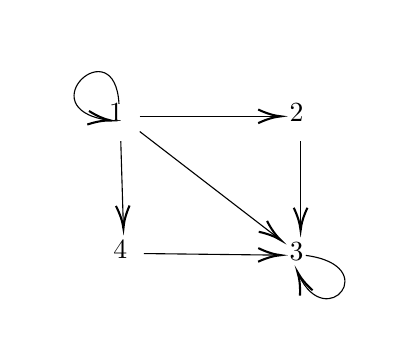
\begin{tikzpicture}[x=0.75pt,y=0.75pt,yscale=-1,xscale=1]
%uncomment if require: \path (0,310); %set diagram left start at 0, and has height of 310

%Curve Lines [id:da4085264026586757] 
\draw    (377,99) .. controls (375.03,62.55) and (333.28,100.82) .. (371.21,106.75) ;
\draw [shift={(373,107)}, rotate = 186.95] [color={rgb, 255:red, 0; green, 0; blue, 0 }  ][line width=0.75]    (10.93,-3.29) .. controls (6.95,-1.4) and (3.31,-0.3) .. (0,0) .. controls (3.31,0.3) and (6.95,1.4) .. (10.93,3.29)   ;
%Curve Lines [id:da07333979302693061] 
\draw    (467,172) .. controls (504.24,176.9) and (477.13,209.65) .. (463.8,181.78) ;
\draw [shift={(463,180)}, rotate = 427.25] [color={rgb, 255:red, 0; green, 0; blue, 0 }  ][line width=0.75]    (10.93,-3.29) .. controls (6.95,-1.4) and (3.31,-0.3) .. (0,0) .. controls (3.31,0.3) and (6.95,1.4) .. (10.93,3.29)   ;


% Text Node
\draw (371,97.4) node [anchor=north west][inner sep=0.75pt]    {$1$};
% Text Node
\draw (458,97.4) node [anchor=north west][inner sep=0.75pt]    {$2$};
% Text Node
\draw (458,164.4) node [anchor=north west][inner sep=0.75pt]    {$3$};
% Text Node
\draw (373,163.4) node [anchor=north west][inner sep=0.75pt]    {$4$};
% Connection
\draw    (464.5,117) -- (464.5,158) ;
\draw [shift={(464.5,160)}, rotate = 270] [color={rgb, 255:red, 0; green, 0; blue, 0 }  ][line width=0.75]    (10.93,-3.29) .. controls (6.95,-1.4) and (3.31,-0.3) .. (0,0) .. controls (3.31,0.3) and (6.95,1.4) .. (10.93,3.29)   ;
% Connection
\draw    (387,105) -- (453,105) ;
\draw [shift={(455,105)}, rotate = 180] [color={rgb, 255:red, 0; green, 0; blue, 0 }  ][line width=0.75]    (10.93,-3.29) .. controls (6.95,-1.4) and (3.31,-0.3) .. (0,0) .. controls (3.31,0.3) and (6.95,1.4) .. (10.93,3.29)   ;
% Connection
\draw    (387,112.32) -- (453.42,163.46) ;
\draw [shift={(455,164.68)}, rotate = 217.6] [color={rgb, 255:red, 0; green, 0; blue, 0 }  ][line width=0.75]    (10.93,-3.29) .. controls (6.95,-1.4) and (3.31,-0.3) .. (0,0) .. controls (3.31,0.3) and (6.95,1.4) .. (10.93,3.29)   ;
% Connection
\draw    (377.86,117) -- (379.08,157) ;
\draw [shift={(379.14,159)}, rotate = 268.26] [color={rgb, 255:red, 0; green, 0; blue, 0 }  ][line width=0.75]    (10.93,-3.29) .. controls (6.95,-1.4) and (3.31,-0.3) .. (0,0) .. controls (3.31,0.3) and (6.95,1.4) .. (10.93,3.29)   ;
% Connection
\draw    (389,171.11) -- (453,171.86) ;
\draw [shift={(455,171.89)}, rotate = 180.67] [color={rgb, 255:red, 0; green, 0; blue, 0 }  ][line width=0.75]    (10.93,-3.29) .. controls (6.95,-1.4) and (3.31,-0.3) .. (0,0) .. controls (3.31,0.3) and (6.95,1.4) .. (10.93,3.29)   ;

\end{tikzpicture}
\end{remark}

